\documentclass{beamer}
\mode<presentation>
\usetheme{CambridgeUS}
\usepackage[russian]{babel}
\usepackage[utf8]{inputenc}
\usepackage[T2A]{fontenc}
\usepackage{sansmathaccent}

\usepackage{verbatim}
\usepackage{alltt}

\pdfmapfile{+sansmathaccent.map}
\title[UX Elements]{Элементы опыта взаимодействия}
\author{Наумов Д.А., доц. каф. КТ}
\date[09.09.2020] {Компьютерная графика и проектирование графических интерфейсов, 2020}

\begin{document}

%ТИТУЛЬНЫЙ СЛАЙД
\begin{frame}
  \titlepage
\end{frame}
  
%СОДЕРЖАНИЕ ЛЕКЦИИ
\begin{frame}
  \frametitle{Содержание лекции}
  \tableofcontents  
\end{frame}

\section{Элементы опыта взаимодействия}
  
\begin{frame}[t]
\begin{block}{Цель освоения дисцпилины}
ознакомление с принципами информационной архитектуры, основами теории проектирования интерфейсов и визуального дизайна.
\end{block}
\begin{block}{Предмет изучения дисцпилины:}
\begin{itemize}
\item информационная архитектура;
\item теория разработки интерфейсов;
\item основы графического дизайна интерфейсов пользователя.
\end{itemize}
\end{block}
\begin{block}{Задачи дисциплины}
\begin{itemize}
\item формирование представлений об информационной архитектуре; 
\item формирование умений анализировать предметную область;
\item выработка навыков проектирования интерфейсных прототипов: 
\item формирование умений использовать элементы визуального дизайна при создании интерфейсов.
\end{itemize}
\end{block}
\end{frame}  

\begin{frame}{Веб-сайт - инструмент самообслуживания}
\begin{figure}[h]
\centering
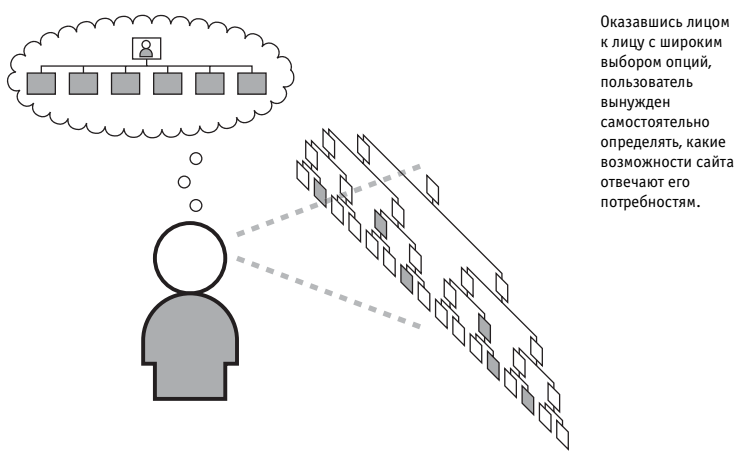
\includegraphics[scale=0.5]{images/lec01-pic01.png}
\end{figure}
\end{frame}

\begin{frame}{Конкурентная борьба и возврат инвестиций}
\begin{figure}[h]
\centering
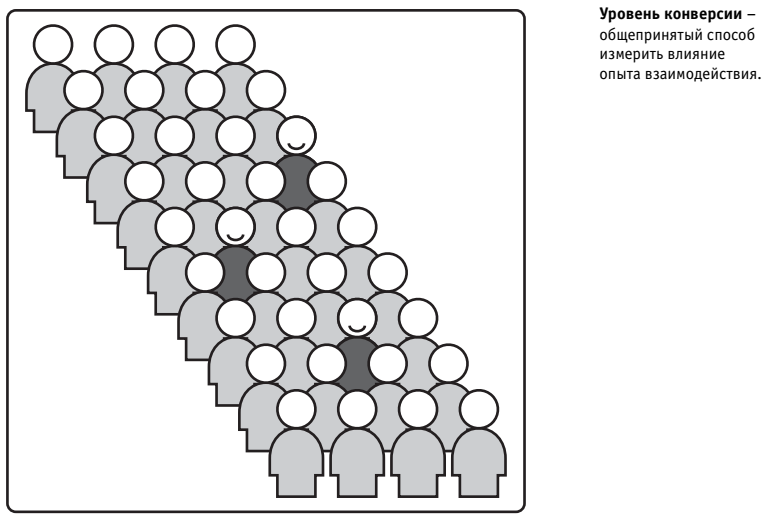
\includegraphics[scale=0.4]{images/lec01-pic02.png}
\end{figure}
\begin{itemize}
\item уровень конверсии; 
\item количество брошенных <<корзин>> с покупками.
\end{itemize}
\end{frame}

\begin{frame}
\begin{figure}[h]
\centering
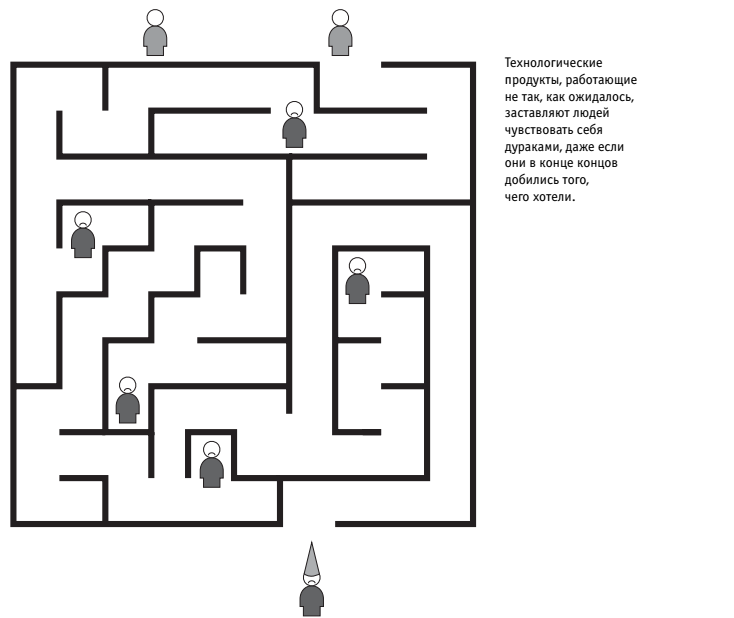
\includegraphics[scale=0.4]{images/lec01-pic03.png}
\end{figure}
Повышение эффективности:
\begin{itemize}
\item помочь работать быстрее;
\item помочь меньше ошибаться.
\end{itemize}
\end{frame}

\section{Пять уровней}

\begin{frame}
  \frametitle{Содержание лекции}
  \tableofcontents[current]
\end{frame}

\begin{frame}
\begin{figure}[h]
\centering

\includegraphics[scale=0.7]{images/lec01-pic04.png}
\end{figure}
\end{frame}

\begin{frame}
\begin{figure}[h]
\centering
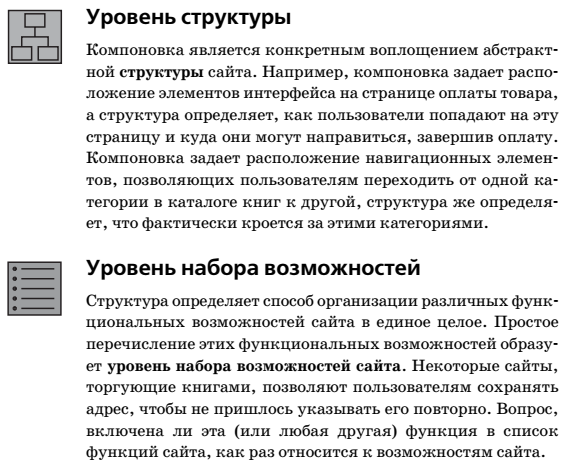
\includegraphics[scale=0.7]{images/lec01-pic05.png}
\end{figure}
\end{frame}

\begin{frame}
\begin{figure}[h]
\centering

\includegraphics[scale=0.7]{images/lec01-pic06.png}
\end{figure}
\end{frame}

\begin{frame}
\begin{figure}[h]
\centering
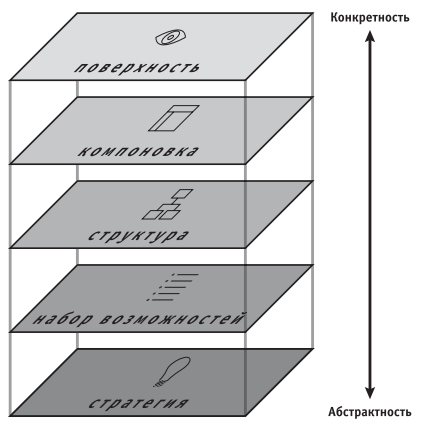
\includegraphics[scale=0.7]{images/lec01-pic07.png}
\end{figure}
\end{frame}

\begin{frame}{Зависимость уровней}
\begin{figure}[h]
\centering
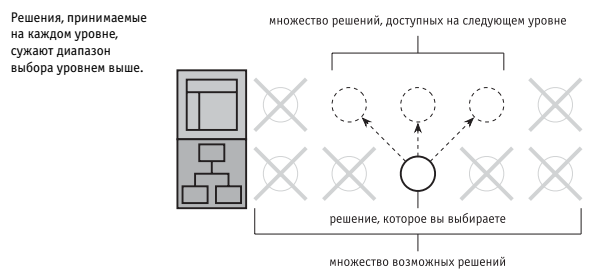
\includegraphics[scale=0.7]{images/lec01-pic08.png}
\end{figure}
\end{frame}

\begin{frame}{Волновой эффект}
\begin{figure}[h]
\centering
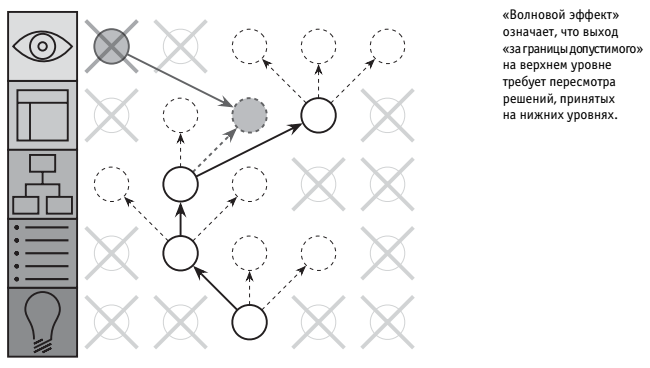
\includegraphics[scale=0.7]{images/lec01-pic09.png}
\end{figure}
\end{frame}

\begin{frame}{Планирование проекта}
\begin{figure}[h]
\centering
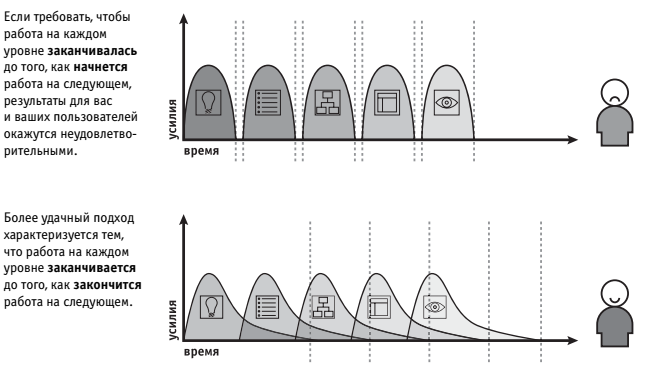
\includegraphics[scale=0.7]{images/lec01-pic10.png}
\end{figure}
\end{frame}

\begin{frame}{Двойственность природы WWW}
\begin{figure}[h]
\centering
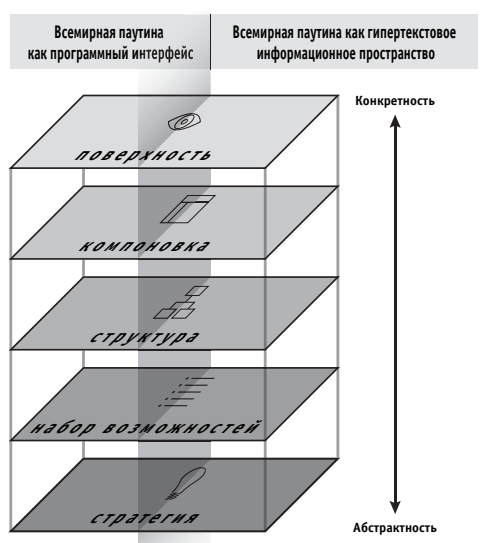
\includegraphics[scale=0.5]{images/lec01-pic11.png}
\end{figure}
\end{frame}

\begin{frame}{Элементы UX: уровень стратегии}
\begin{itemize}
\item Потребности пользователей - это цели сайта, источник которых находится за границами нашей организации;
\item Цели сайта - собственные цели (бизнес-цели или иные).
\end{itemize}
\begin{figure}[h]
\centering
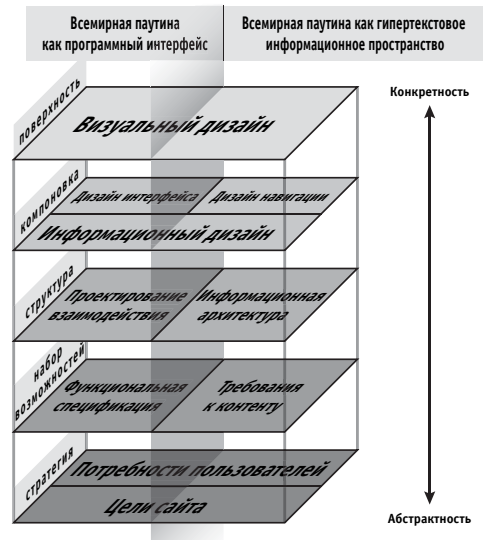
\includegraphics[scale=0.4]{images/lec01-pic12.png}
\end{figure}
\end{frame}

\begin{frame}{Элементы UX: уровень набора возможностей}
\begin{itemize}
\item функциональная спецификация - описание функциональных возможностей;
\item требования к контенту - описание элементов, которые надо создать.
\end{itemize}
\begin{figure}[h]
\centering
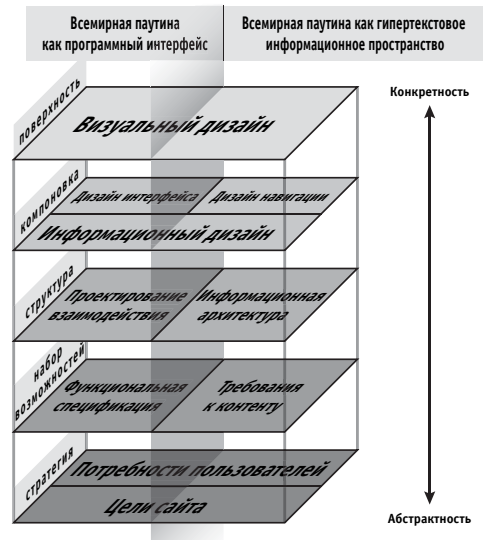
\includegraphics[scale=0.4]{images/lec01-pic12.png}
\end{figure}
\end{frame}

\begin{frame}{Элементы UX: уровень структуры}
\begin{itemize}
\item проектирование взоимодействия - как система будет вести себя в ответ на действия пользователей;
\item информационная архитектура - организация элементов содержимого.
\end{itemize}
\begin{figure}[h]
\centering
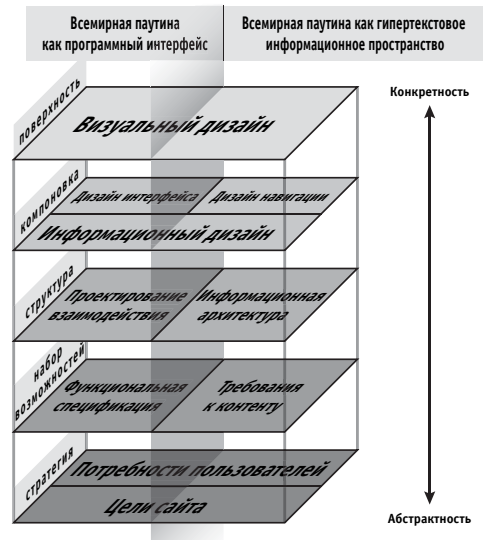
\includegraphics[scale=0.4]{images/lec01-pic12.png}
\end{figure}
\end{frame}

\begin{frame}{Элементы UX: уровень компоновки}
\begin{itemize}
\item информационный дизайн - представление информации, облегчающее восприятие;
\item дизайн интерфейса - организация взаимодействия с пользователем;
\item дизайн навигации - перемещение по информационной архитектуре.
\end{itemize}
\begin{figure}[h]
\centering
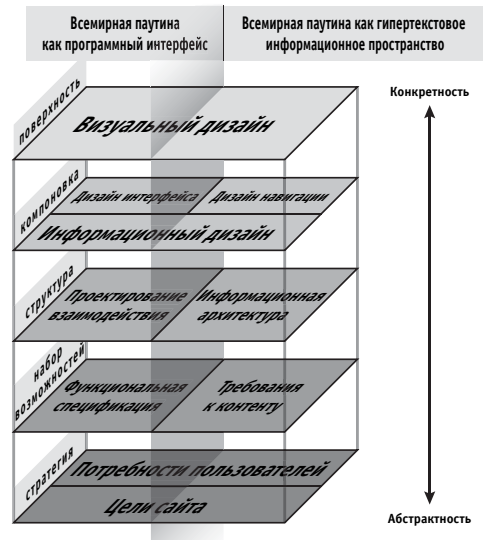
\includegraphics[scale=0.4]{images/lec01-pic12.png}
\end{figure}
\end{frame}

\begin{frame}{Элементы UX: уровень поверхности}
\begin{itemize}
\item визуальный дизайн - внешний вид конечного продукта;
\end{itemize}
\begin{figure}[h]
\centering
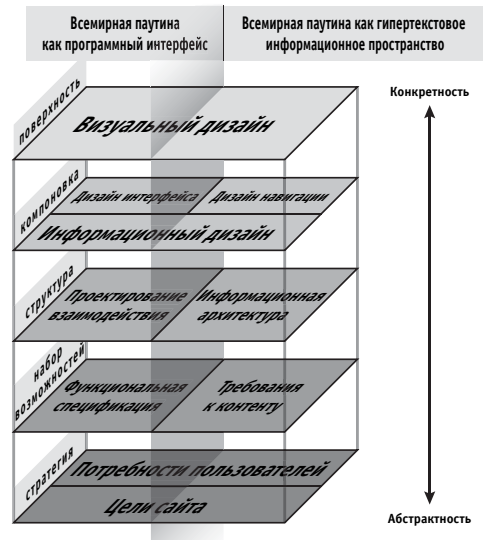
\includegraphics[scale=0.4]{images/lec01-pic12.png}
\end{figure}
\end{frame}

\section{Уровень стратегии}
\begin{frame}
  \frametitle{Содержание лекции}
  \tableofcontents[current]
\end{frame}

\begin{frame}{Уровень стратегии}
\begin{figure}[h]
\centering
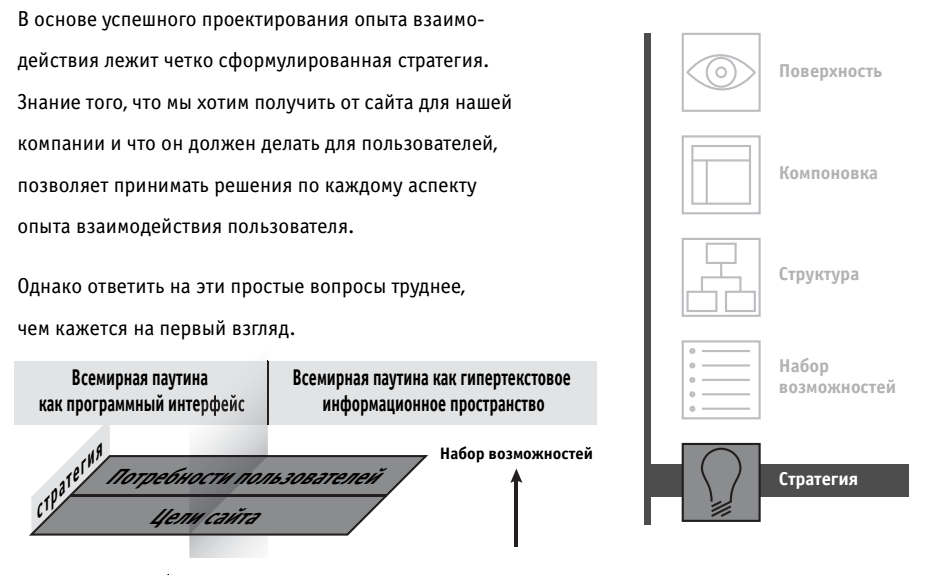
\includegraphics[scale=0.4]{images/lec01-pic13.png}
\end{figure}
\begin{itemize}
\item Что хотим получить от нашего сайта мы?
\item Что хотят получить от него наши пользователи?
\end{itemize}
\end{frame}

\begin{frame}{Уровень стратегии}
\begin{itemize}
\item Что хотим получить от нашего сайта мы? Ответив, мы получим \textbf{цели сайта}. 
	\begin{itemize}
	\item бизнес-цели
	\begin{itemize}
		\item заработать больше денег?
		\item съэкономить?		
		\item предоставить пользователям инструмент для общения в реальном времени, основанный на технологии Java?		
	\end{itemize}
	\item идентичность бренда
	\end{itemize}
\item Что хотят получить от него наши пользователи? Ответив, мы получим \textbf{описание потребностей пользователя}. 
\end{itemize}
\end{frame}

\begin{frame}
\begin{block}{Метрики успешности}
понимаются индикаторы, за которыми мы следим после появления сайта в Интернете, чтобы понять, насколько он соответствует нашим целям
и потребностям наших пользователей. 
\end{block}
\begin{figure}[h]
\centering
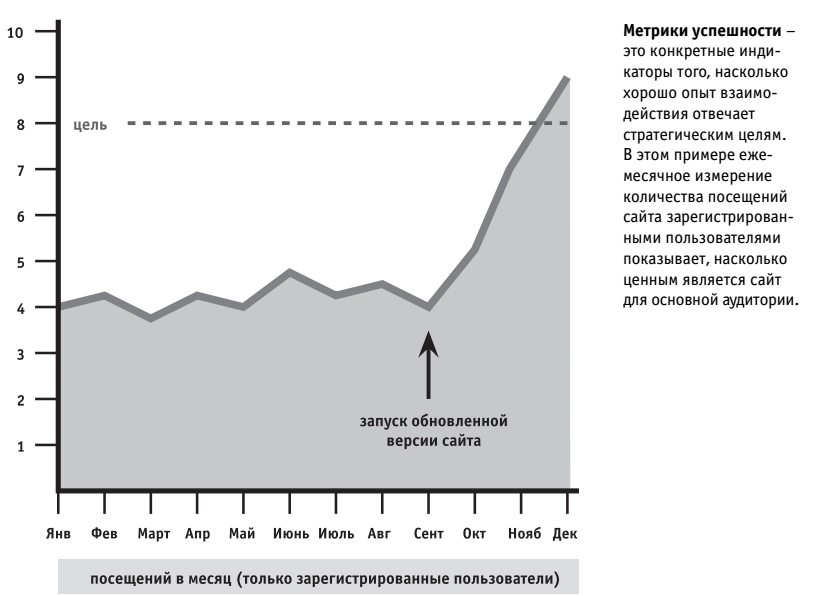
\includegraphics[scale=0.4]{images/lec01-pic14.png}
\end{figure}
\end{frame}

\begin{frame}
\begin{itemize}
\item сколько времени проводит средний пользователь на вашем сайте в течение каждого посещения?
\item для сайтов, рассчитывающих на доход от рекламы: количество просмотров страниц - число запросов той или иной страницы в течение дня.
\item косвенные показатели: если сайт предоставляет клиентам решения типичных проблем, возникающих при использовании вашей
продукции, количество звонков в службу поддержки клиентов должно сократиться.
\end{itemize}
Хорошие метрики
\begin{itemize}
\item влияют на решения, принимаемые по ходу работы над проектом, 
\item дают вам в руки конкретное свидетельство ценности опыта взаимодействия.
\item такая метрика, любое изменение которой можно легко привязать к опыту взаимодействия пользователя с сайтом. 
\end{itemize}
\end{frame}

\begin{frame}
Кто пользователь нашего сайта?
\begin{figure}[h]
\centering
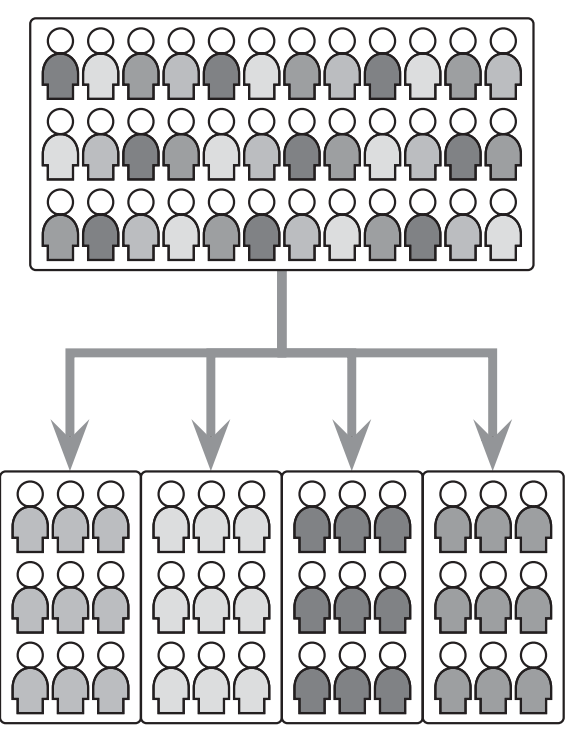
\includegraphics[scale=0.25]{images/lec01-pic15.png}
\end{figure}
Сегментация аудитории:
	\begin{itemize}
	\item по демографическим критериям (пол, возраст, образование, семейное положение, доход);
	\item по психографическим критериями (как пользователи воспринимают окружающий мир в целом или конкретную тему вашего сайта).
	\end{itemize}
\end{frame}

\begin{frame}
\begin{block}{Usability (исследование пользовательской аудитории)}
\begin{itemize}
\item тестирование проекта на репрезентативной группе пользователей;
\item следование одной совершенно конкретной методологии проектирования взаимодействия;
\item стремление сделать продукты простыми в использовании.
\end{itemize}
\end{block}
Исследование пользовательской аудитории состоит в сборе данных, позволяющих понять, кто является пользователем нашего продукта.
\begin{itemize}
\item маркетинговые исследования - фокусируются на понимании поведения, желаний и предпочтений пользователей;
\item контекстуальные исследования -  набор методов, которые позволят понять пользователей в контексте их повседневной жизни;
\item анализ задачи пользователя - метод подробного изучения шагов, предпринимаемых пользователями при решении своих задач;
\item пользовательское тестирование - тестирование вашего продукта пользователями (или прототипов продукта).
\end{itemize}
\end{frame}

\begin{frame}{Персонажи (профили пользователей)}
\begin{block}{Персонаж}
это вымышленный герой, который представ ляет потребности целой группы реальных пользователей.
\end{block}
\begin{figure}[h]
\centering
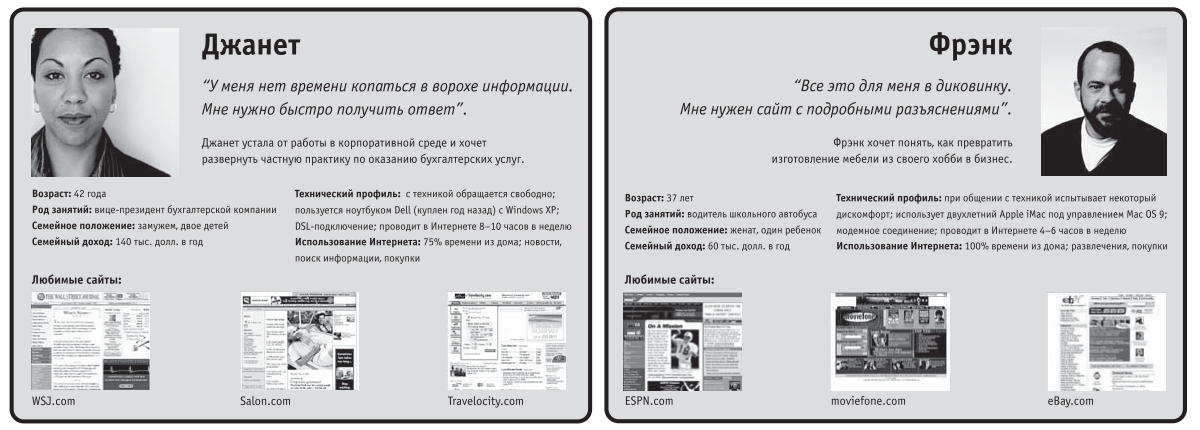
\includegraphics[scale=0.35]{images/lec01-pic16.png}
\end{figure}
\end{frame}

\begin{frame}{Что читать по данной теме?}
\begin{enumerate}
\item Гарретт Дж.  Веб-дизайн. Книга Дж. Гарретта. Элементы опыта взаимодействия. – М.: Символ-Плюс, 2008. – 192 с.
\item Алан Купер <<Психбольница в руках пациентов, или почему высокие технологии сводят нас с ума и как восстановить душевное равновесие>>. – Пер. с англ. – СПб.: Символ Плюс, 2004.
\item Стив Круг <<Веб-дизайн: книга Стива Круга, или <<не заставляйте меня думать!>>, 2-е издание. – Пер. с англ. – СПб.: Символ-Плюс, 2008.
\end{enumerate}
\end{frame}

%\section{Уровень набора возможностей}
%\section{Уровень структуры}
%\section{Уровень компоновки}
%\section{Уровень поверхности}

\end{document}
